\chapter{Production Plan}
\label{ch:prod_plan}

In case the finalised concept will be produced by series production, a production plan will come in handy to show the required activities to build the aircraft. The production plan shows, in general lines, which steps need to be taken into building the aircraft, and which steps can be done concurrently. \autoref{fig:pp_top} shows the production plan for The Winged Quadcopter.

\begin{figure}[H]
    \centering
    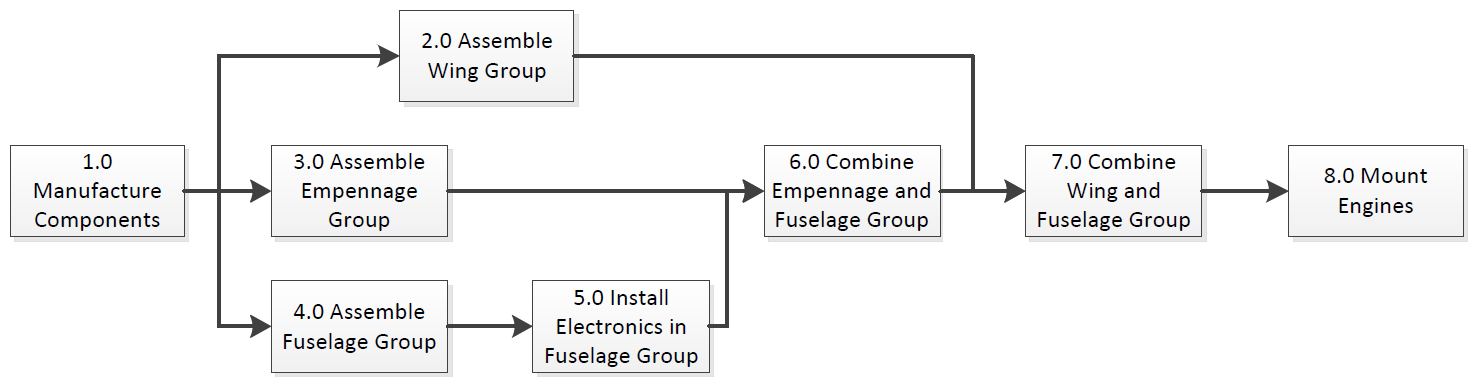
\includegraphics[width=\textwidth]{ProductionPlan/Figures/pp_top}
    \caption{Top Level Production Flow Diagram}
    \label{fig:pp_top}
\end{figure}

Looking at the top level, all of the required parts are manufactured first. Next, the three main groups of the aircraft can be constructed simultaneously, namely the fuselage, empennage and wing. Once these are constructed the assembly can begin, starting with the fuselage and the empennage, followed by the wing. This order has been chosen because the wings will complicate the process by taking up a lot of space. Tthe engines are mounted last in order to minimise the risk of damaging them or the UAV during production.

Each assembly stage presented in the top level is shown in detail below, starting with the wing assembly, \autoref{fig:pp_2}. Here, the wing structure is constructed by first creating a base for all other components to be fixed to. The exact type of base will be determined at a further development stage, depending on the materials used. Next, parts such as control surfaces or engine mounts are constructed and mounted onto the base. Finally, an outer layer is added for various purposes such as strength or protection. Again, this will depend on the materials chosen.

\begin{figure}[H]
    \centering
    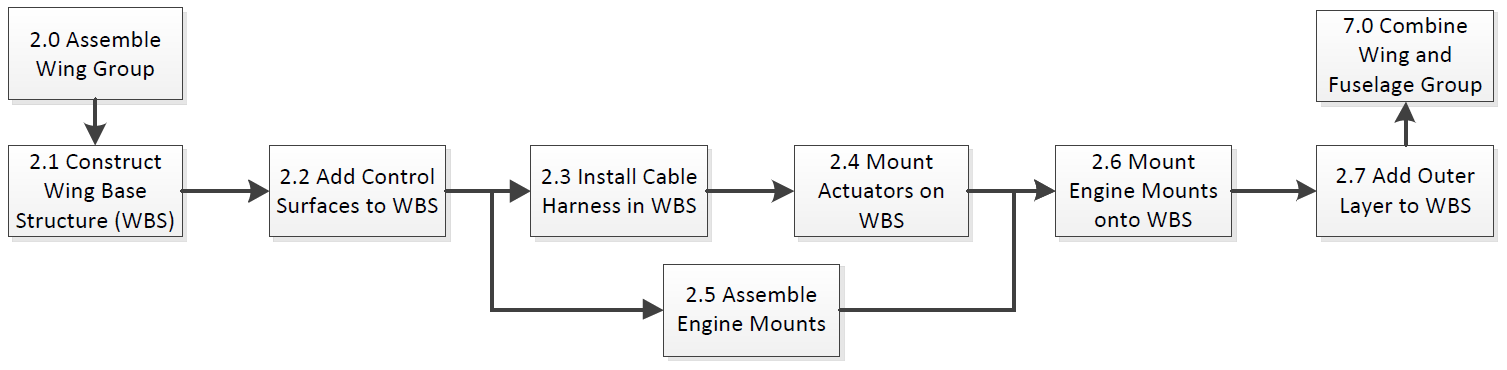
\includegraphics[width=\textwidth]{ProductionPlan/Figures/pp_2}
    \caption{Wing Assembly Flow Diagram}
    \label{fig:pp_2}
\end{figure}

The detailed empennage assembly is shown in \autoref{fig:pp_3}. This production stage comprises three parallel processes, namely the construction of the vertical and horizontal stabilisers, as well as of the empennage base. These are then assembled together, after which the actuators are mounted onto the base and connected to the control surfaces. The stage ends with the addition of an outer layer to the entire empennage.

\begin{figure}[H]
    \centering
    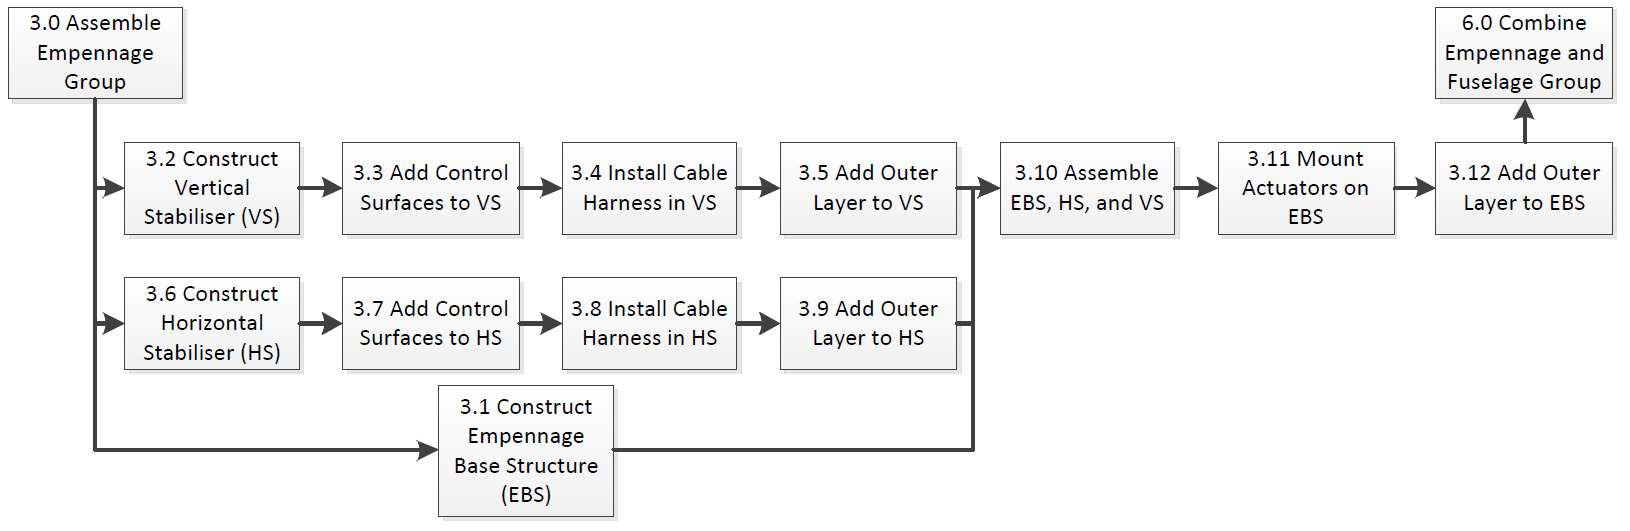
\includegraphics[width=\textwidth]{ProductionPlan/Figures/pp_3}
    \caption{Empennage Assembly Flow Diagram}
    \label{fig:pp_3}
\end{figure}

The construction of the fuselage is split into two stages, namely the structural assembly (\autoref{fig:pp_4}) and the installation of the electronics in the fuselage (\autoref{fig:pp_5}). The first stage consists of constructing the fuselage base and payload bay in parallel, and then assembling them together. The undercarriage is mounted afterwards making it easier to assemble the payload bay beforehand. With the undercarriage installed, from this stage on the UAV will not require any additional structural supports during production. Finally, the engine mounts are attached to the fuselage. 

\begin{figure}[H]
    \centering
    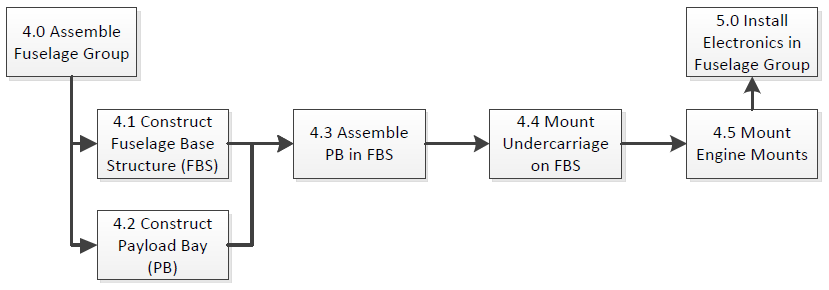
\includegraphics[width=0.8\textwidth]{ProductionPlan/Figures/pp_4}
    \caption{Fuselage Structure Assembly Flow Diagram}
    \label{fig:pp_4}
\end{figure}

The second stage consists of installing the cabling and the control computer first. The control computer will make it possible to test all the electrical components on the UAV, such as the actuators or motors. Performing these tests immediately after the installation of each electrical component will make it easier to fix or replace them if needed. Next the sensors and communication system are mounted on the fuselage.

\begin{figure}[H]
    \centering
    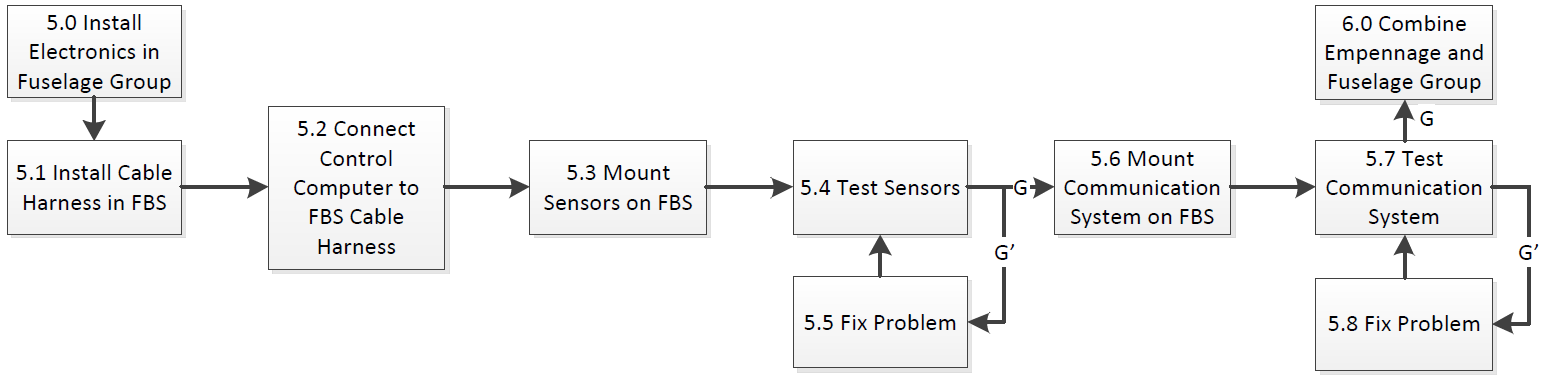
\includegraphics[width=\textwidth]{ProductionPlan/Figures/pp_5}
    \caption{Fuselage Electronics Assembly Flow Diagram}
    \label{fig:pp_5}
\end{figure}

Next, the empennage is assembled with the fuselage first (\autoref{fig:pp_6}), followed by the assembly of the fuselage with the wings(\autoref{fig:pp_7}). Both these processes consist of joining the structures, connecting the cable harnesses, and testing all the connections and actuators. The only exception is that during the fuselage-empennage stage, an outer layer is finally added to the fuselage structure. Delaying this step makes it easier to connect the structures and install all electronic components.

\begin{figure}[H]
    \centering
    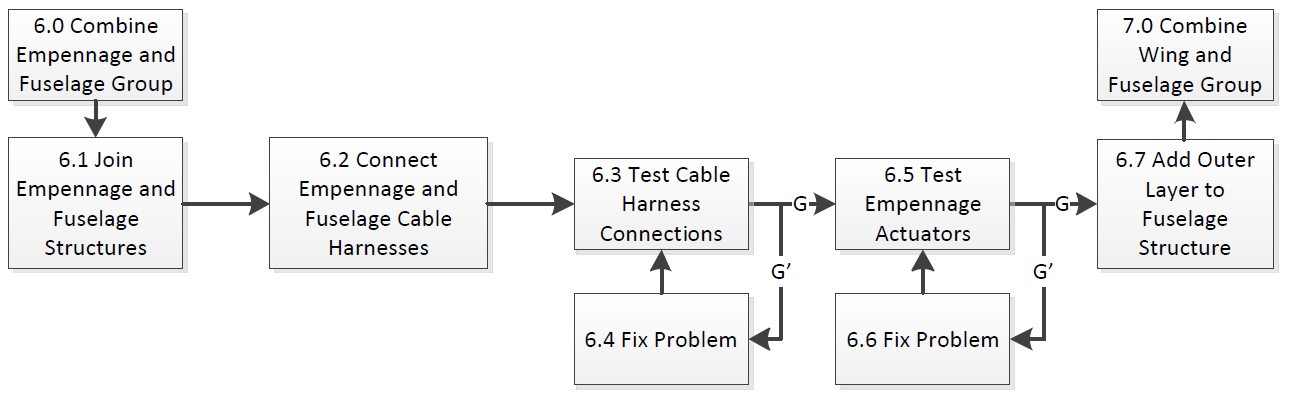
\includegraphics[width=0.9\textwidth]{ProductionPlan/Figures/pp_6}
    \caption{Fuselage and Empennage Joining Flow Diagram}
    \label{fig:pp_6}
\end{figure}

\begin{figure}[H]
    \centering
    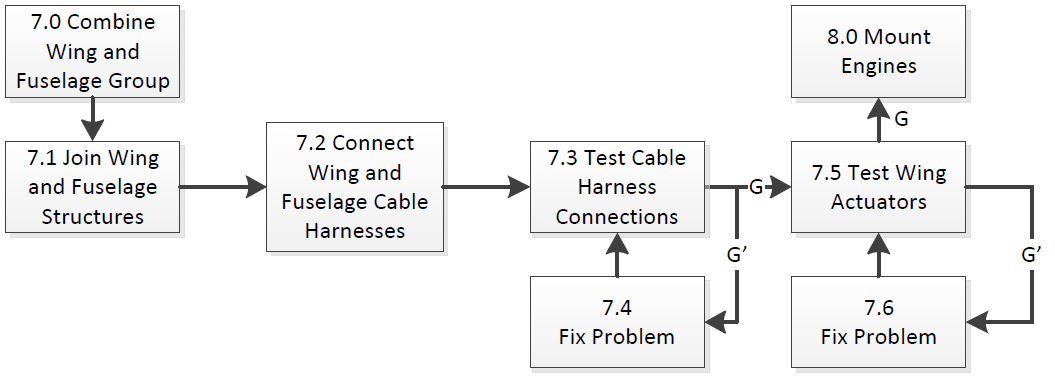
\includegraphics[width=0.8\textwidth]{ProductionPlan/Figures/pp_7}
    \caption{Fuselage and Wing Joining Flow Diagram}
    \label{fig:pp_7}
\end{figure}

The last step (\autoref{fig:pp_8}) involves mounting the engines to the wings and fuselage. It is assumed that the engines will be heavy, hence attaching them last will make it easier to handle the product during the preceding production stages. In addition, there will be a lesser risk of damaging the UAV or the engines themselves during improper handling.

\begin{figure}[H]
    \centering
    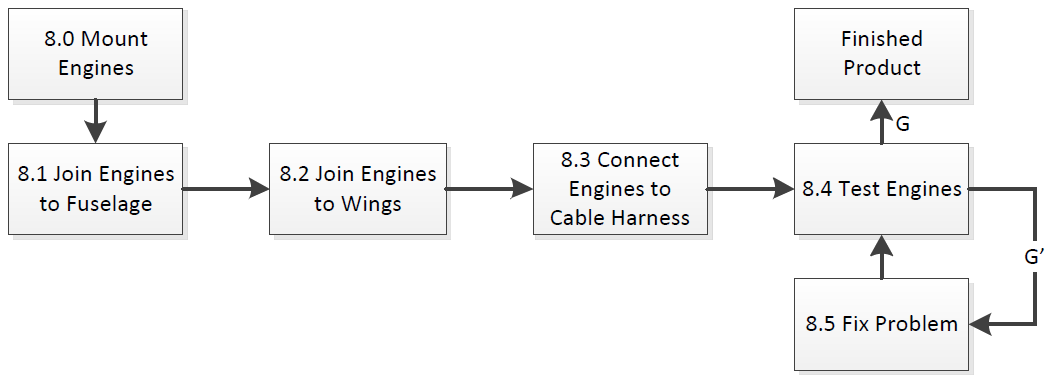
\includegraphics[width=0.8\textwidth]{ProductionPlan/Figures/pp_8}
    \caption{Engine Mounting Flow Diagram}
    \label{fig:pp_8}
\end{figure}

%Constructing the wings will be straightforward. The empennage however has some concurrent construction going on, the assembly of the three pieces must be done in a specific order because the empennage is a T-tail. The order has been chosen to first assemble the base and the vertical tail, followed by the horizontal tail. WRITE LATER WHEN WE KNOW MORE ABOUT G